\documentclass[11pt,a4paper]{article}
\usepackage[margin=1in]{geometry}
\usepackage{graphicx}
\usepackage{amsmath}
\usepackage{array}
\usepackage[section]{placeins}
\usepackage[hidelinks]{hyperref}
\hypersetup{pdftitle={Programming Assignment 2: Final Report},pdfauthor={2024ADPS0831G}}
\pagestyle{plain}
\setcounter{topnumber}{3}
\setcounter{bottomnumber}{3}
\setcounter{totalnumber}{5}
\renewcommand{\topfraction}{0.9}
\renewcommand{\bottomfraction}{0.9}
\renewcommand{\textfraction}{0.1}
\renewcommand{\floatpagefraction}{0.7}
\begin{document}
\title{Programming Assignment 2: Final Report}
\author{2024ADPS0831G}
\date{}
\maketitle

\section{Introduction / Objective}

The task is six-class classification from 24 sensor measurements. The supplied split contains 1,800 training and 1,800 validation examples. The experiments below isolate the requested training choices before selecting one model for retraining on all 3,600 examples.


\section{Experimental Setup}

\begin{table}[htbp]
\centering
\setlength{\tabcolsep}{4pt}
\renewcommand{\arraystretch}{1.12}
\normalsize
\begin{tabular}{@{}>{\raggedright\arraybackslash}p{117.04pt} >{\raggedright\arraybackslash}p{326.23pt}@{}}
\hline
Common setting & Value \\
\hline
Optimizer / mini-batch & SGD, momentum 0 / batch size 64 \\
Duration / random seed & 120 epochs for every controlled run / 831031 \\
Input scaling & Original training.csv mean and population standard deviation (ddof=0) \\
Biases / output & Zero initialization / six logits, with no output activation \\
\hline
\end{tabular}
\caption{Common experimental settings.}
\end{table}

Every run starts from scratch. Model initialization and mini-batch shuffling have separately reset generators using the same seed. Same-shaped models in Parts A and B have exactly matching starting parameters. Losses are measured on the complete datasets after each epoch and exclude the L2 penalty. No validation examples enter the controlled-run gradient updates.


\section{Part A - Effect of Activation Function}

Architecture 24-32-6; cross-entropy; learning rate 0.05; weight decay 0. All weights use Nielsen initialization: normal standard deviation 1/sqrt(fan-in).


\begin{figure}[htbp]
\centering
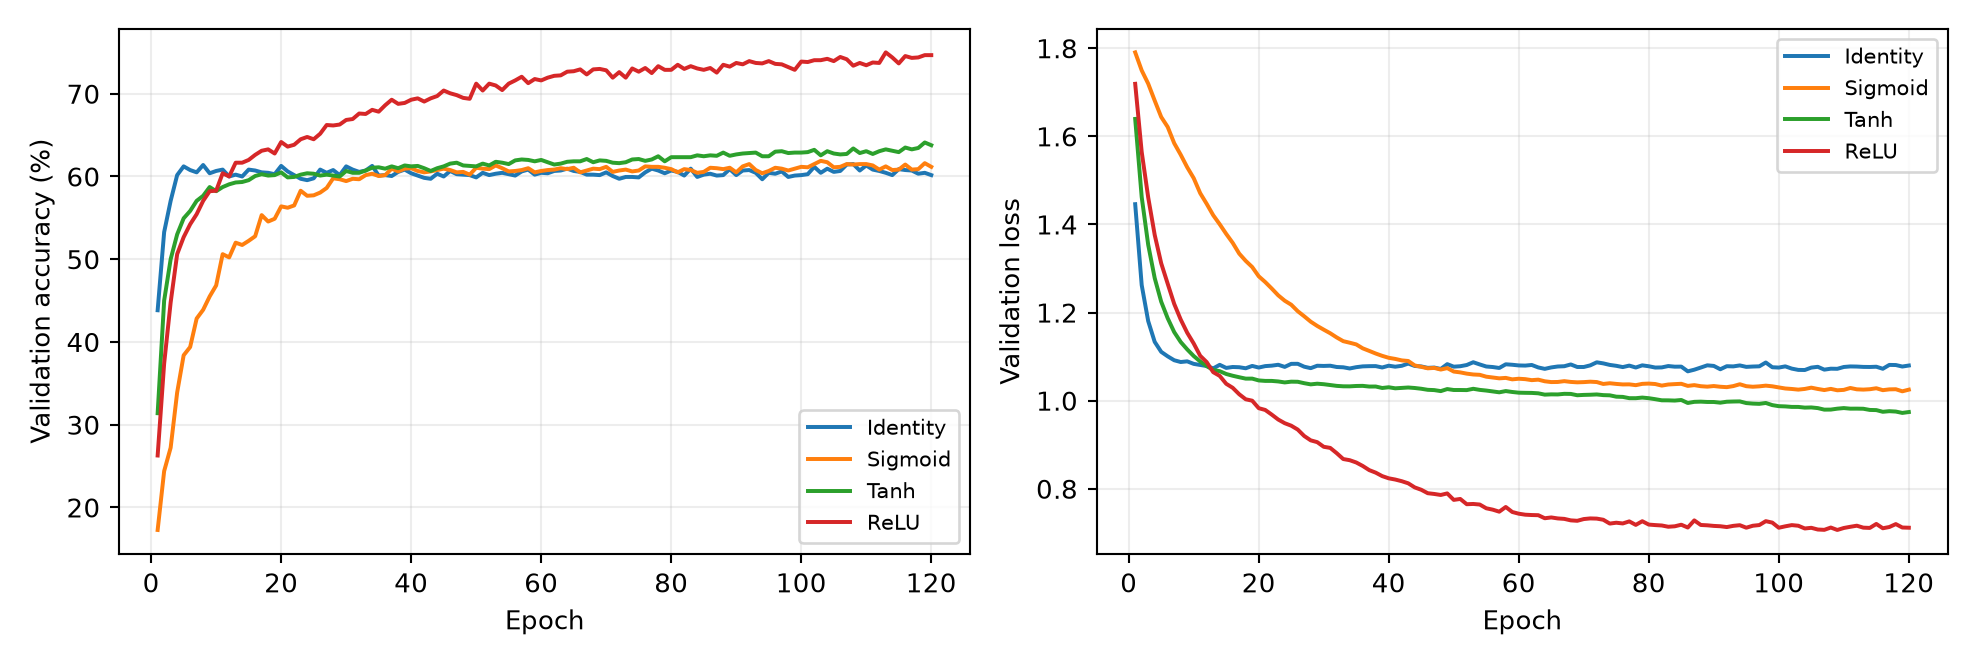
\includegraphics[width=1.0000\linewidth]{results/figures/A_activation.png}

\caption{Validation accuracy and cross-entropy for the four hidden activations.}
\end{figure}

\begin{table}[htbp]
\centering
\setlength{\tabcolsep}{4pt}
\renewcommand{\arraystretch}{1.12}
\small
\begin{tabular}{@{}>{\raggedright\arraybackslash}p{65.60pt} >{\raggedright\arraybackslash}p{94.31pt} >{\raggedright\arraybackslash}p{53.30pt} >{\raggedright\arraybackslash}p{106.61pt} >{\raggedright\arraybackslash}p{99.45pt}@{}}
\hline
Activation & Best val. accuracy (\%) & Best epoch & Final val. accuracy (\%) & Final val. CE \\
\hline
Identity & 61.50 & 108 & 60.17 & 1.080 \\
Sigmoid & 61.89 & 103 & 61.17 & 1.025 \\
Tanh & 64.11 & 119 & 63.78 & 0.974 \\
ReLU & 75.00 & 113 & 74.67 & 0.712 \\
\hline
\end{tabular}
\caption{Effect of hidden activation on validation performance.}
\end{table}

Identity improves quickly but levels off near 60\%, consistent with its overall linear decision function. Sigmoid learns more slowly and ends close to that baseline; tanh makes a modest improvement. ReLU continues improving and reaches 75.00\% at its best checkpoint. This run supports nonlinear features, particularly ReLU, for this dataset; it does not establish that every nonlinear activation will outperform a linear model under every training setup.


\section{Part B - Cross-Entropy versus Quadratic Cost}

Both runs use 24-32-6, ReLU, Kaiming normal initialization, learning rate 0.05 and zero weight decay. They start with identical parameters and process the same mini-batches in the same order. Only the training objective changes.


Cross-entropy receives the logits directly. The quadratic objective uses softmax probabilities and one-hot targets, with reduction:\newline \textbf{Q = (1 / 2n) sum over examples i and classes k of (p\textsubscript{ik} - y\textsubscript{ik})\textsuperscript{2}.}\newline The sum is over the six classes, followed by the mean over examples. There is no extra division by six.


\begin{figure}[htbp]
\centering
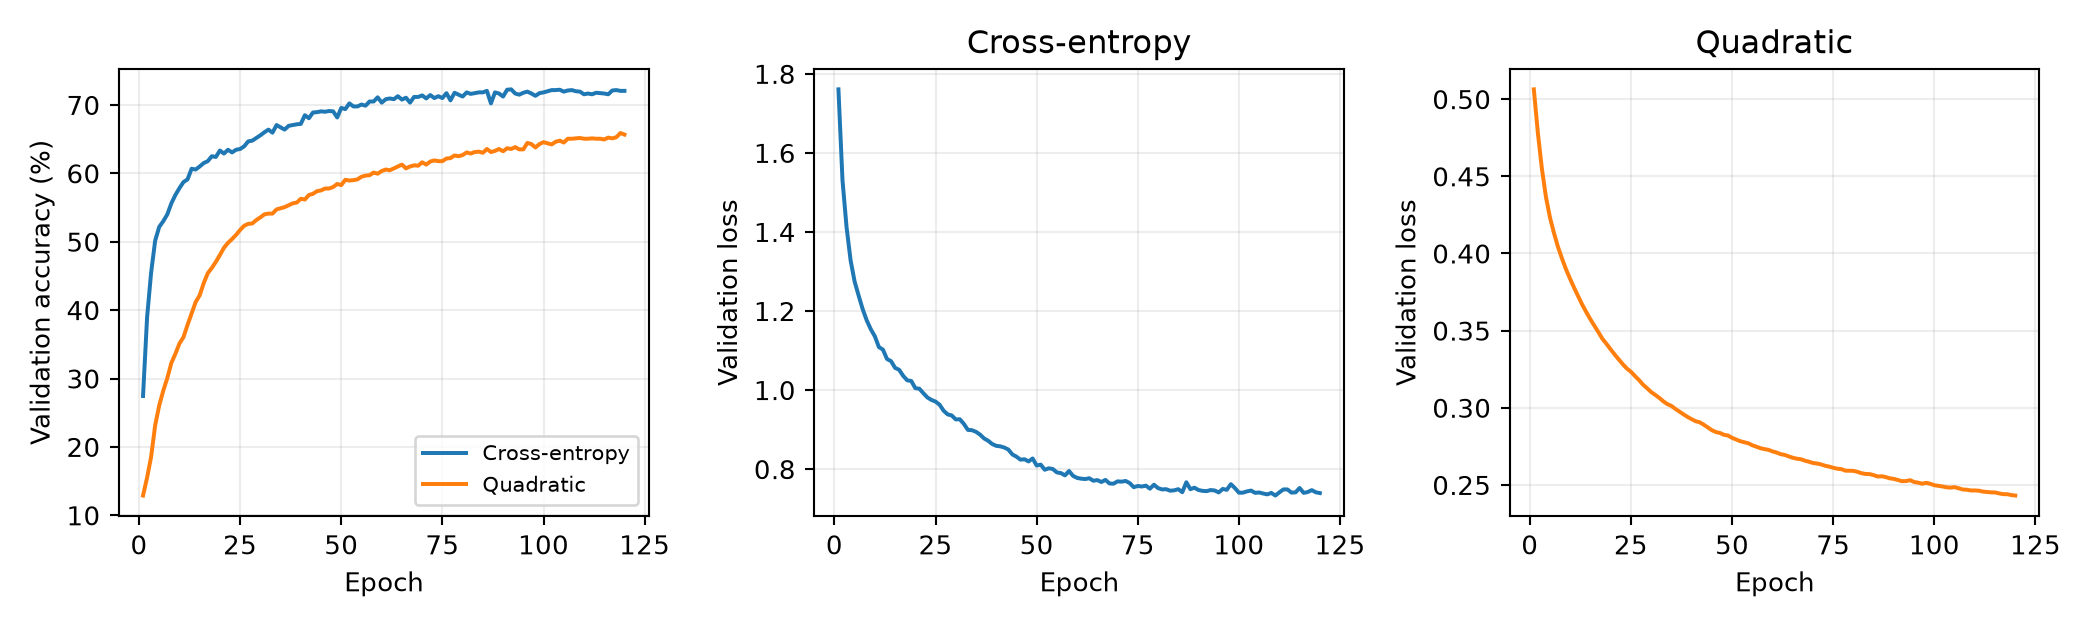
\includegraphics[width=1.0000\linewidth]{results/figures/B_loss.png}

\caption{Shared accuracy comparison; each objective has its own validation-loss panel and scale.}
\end{figure}

\begin{table}[htbp]
\centering
\setlength{\tabcolsep}{4pt}
\renewcommand{\arraystretch}{1.12}
\small
\begin{tabular}{@{}>{\raggedright\arraybackslash}p{67.57pt} >{\raggedright\arraybackslash}p{76.42pt} >{\raggedright\arraybackslash}p{48.26pt} >{\raggedright\arraybackslash}p{80.44pt} >{\raggedright\arraybackslash}p{80.44pt} >{\raggedright\arraybackslash}p{58.14pt}@{}}
\hline
Objective & Best val. accuracy (\%) & Best epoch & Final train accuracy (\%) & Final val. accuracy (\%) & Final own loss \\
\hline
Cross-entropy & 72.28 & 92 & 88.06 & 72.06 & 0.739 \\
Quadratic & 65.89 & 119 & 73.00 & 65.67 & 0.243 \\
\hline
\end{tabular}
\caption{Cross-entropy and quadratic cost; each loss is reported on its own scale.}
\end{table}

At epoch 20, cross-entropy reaches 63.33\% validation accuracy, compared with 48.06\% for quadratic cost. At epoch 120 the gap remains 6.39 percentage points. Quadratic cost is still improving toward the end of its run, but it has not caught up within the required budget.


This difference is consistent with the objectives having different gradients. For softmax cross-entropy the logit gradient is proportional to p-y. Quadratic cost differentiates through the softmax Jacobian as well, which can weaken updates for confident mistakes. With the learning rate held fixed, the observed learning speed favors cross-entropy. A separate learning-rate search for quadratic cost was not part of this controlled comparison.


The numerical loss values in the last column have different meanings and scales. The quadratic value is not evidence that it is the better model; accuracy and the progress within each curve provide the appropriate comparisons here.


\section{Part C - Effect of Weight Initialization}

Architecture 24-64-32-6; ReLU; cross-entropy; learning rate 0.03; weight decay 0. All layers, including the output layer, use the specified initialization. The normal standard deviations are 0.01, 1, and 1/sqrt(fan-in); Kaiming uses fan-in mode for ReLU.


\begin{figure}[htbp]
\centering
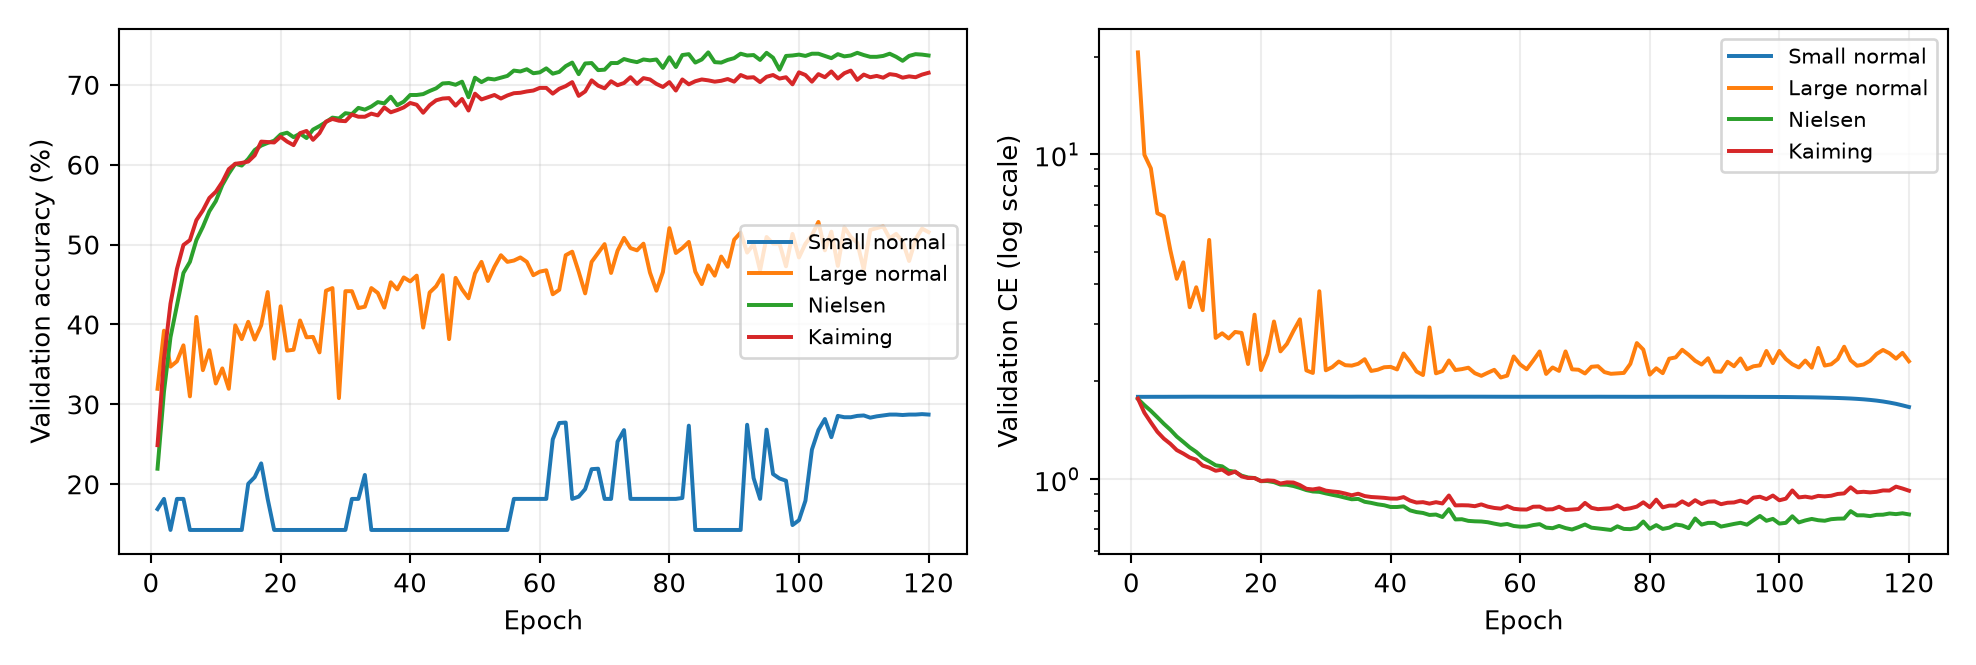
\includegraphics[width=1.0000\linewidth]{results/figures/C_initialization.png}

\caption{Complete validation trajectories. Large-normal initialization starts with much higher loss.}
\end{figure}

\begin{figure}[htbp]
\centering
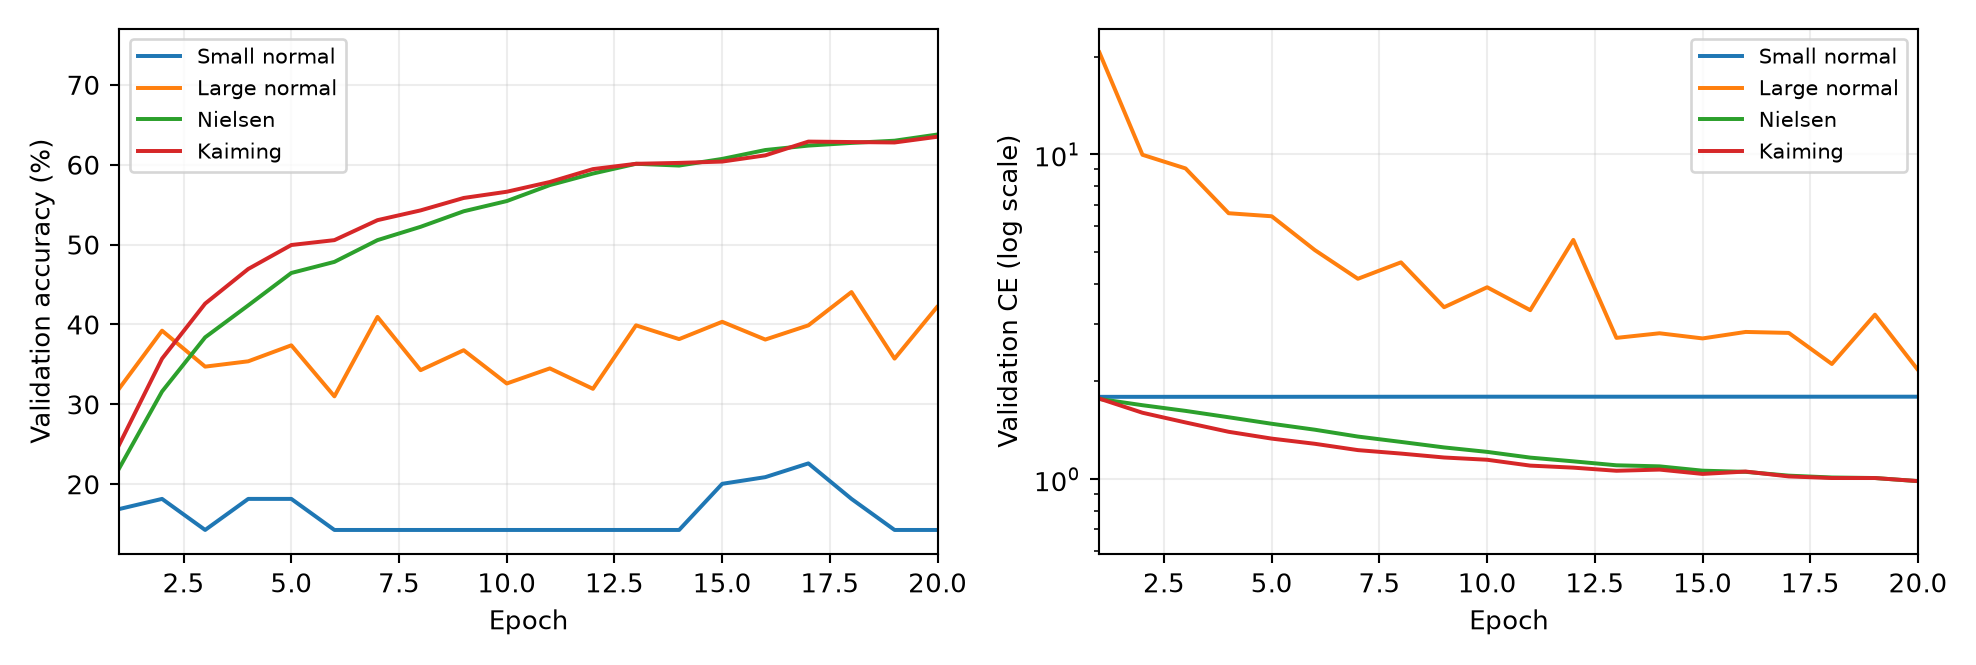
\includegraphics[width=1.0000\linewidth]{results/figures/C_early.png}

\caption{The same runs restricted to epochs 1-20 to show the initial learning behavior.}
\end{figure}

\begin{table}[htbp]
\centering
\setlength{\tabcolsep}{4pt}
\renewcommand{\arraystretch}{1.12}
\small
\begin{tabular}{@{}>{\raggedright\arraybackslash}p{82.01pt} >{\raggedright\arraybackslash}p{73.81pt} >{\raggedright\arraybackslash}p{90.21pt} >{\raggedright\arraybackslash}p{86.11pt} >{\raggedright\arraybackslash}p{87.15pt}@{}}
\hline
Initialization & Epoch 1 val. CE & Epoch 5 val. acc. (\%) & Best val. acc. (\%) & Final val. acc. (\%) \\
\hline
Small normal & 1.792 & 18.17 & 28.78 & 28.72 \\
Large normal & 20.630 & 37.39 & 52.83 & 51.56 \\
Nielsen & 1.765 & 46.44 & 74.06 & 73.67 \\
Kaiming & 1.770 & 49.94 & 71.78 & 71.50 \\
\hline
\end{tabular}
\caption{Early and final validation performance for the initialization comparison.}
\end{table}

Small-normal weights make very little early progress: validation loss stays close to ln(6) and final accuracy is only 28.72\%. Large-normal weights start with validation CE 20.630; the run stays finite but ends at CE 2.306 and 51.56\% accuracy. Fan-in scaling avoids these extremes. Kaiming learns faster at first, while Nielsen finishes better in this fixed-seed run (73.67\% versus 71.50\%). Thus the fastest start did not give the best final validation result.


\section{Part D - Effect of Network Capacity}

ReLU, cross-entropy, Kaiming normal initialization, learning rate 0.03 and zero weight decay are fixed. Increasing capacity greatly reduces training error, but the validation improvement is much smaller.


\begin{table}[htbp]
\centering
\setlength{\tabcolsep}{4pt}
\renewcommand{\arraystretch}{1.12}
\small
\begin{tabular}{@{}>{\raggedright\arraybackslash}p{100.55pt} >{\raggedright\arraybackslash}p{56.31pt} >{\raggedright\arraybackslash}p{72.40pt} >{\raggedright\arraybackslash}p{68.37pt} >{\raggedright\arraybackslash}p{56.31pt} >{\raggedright\arraybackslash}p{57.33pt}@{}}
\hline
Model / hidden layers & Parameters & Train acc. (\%) & Val. acc. (\%) & Train CE & Val. CE \\
\hline
Tiny / 8 & 254 & 68.67 & 64.56 & 0.836 & 0.971 \\
Small / 32 & 998 & 83.28 & 71.22 & 0.475 & 0.758 \\
Medium / 64-32 & 3,878 & 97.83 & 71.50 & 0.132 & 0.921 \\
Large / 128-128 & 20,486 & 99.94 & 72.89 & 0.042 & 0.922 \\
\hline
\end{tabular}
\caption{Network capacity comparison. All metrics are from epoch 120.}
\end{table}

\begin{figure}[htbp]
\centering
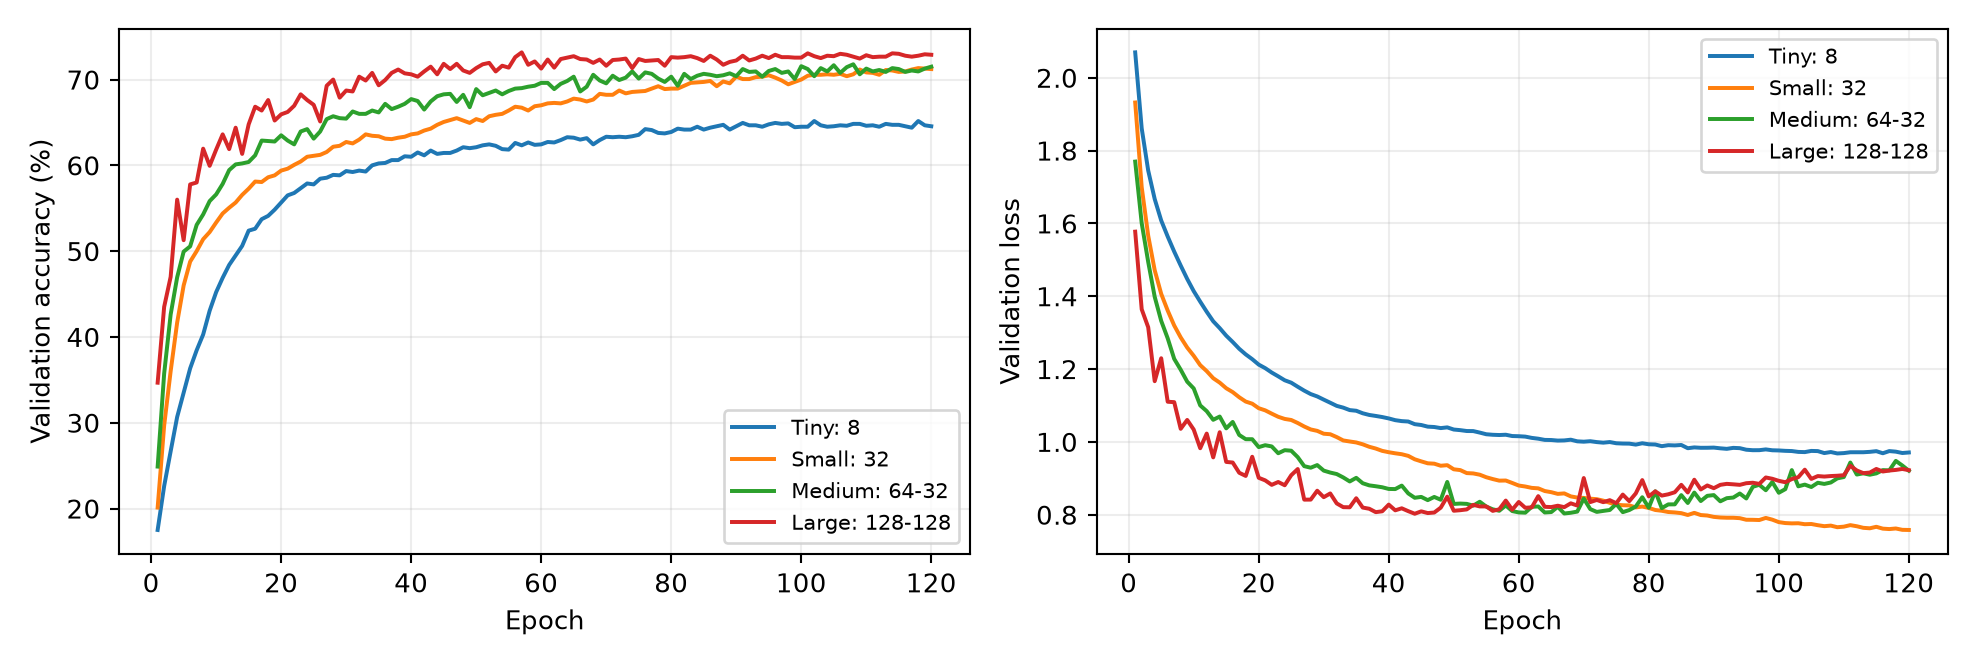
\includegraphics[width=1.0000\linewidth]{results/figures/D_capacity.png}

\caption{Validation accuracy and cross-entropy as network size increases.}
\end{figure}

\begin{figure}[htbp]
\centering
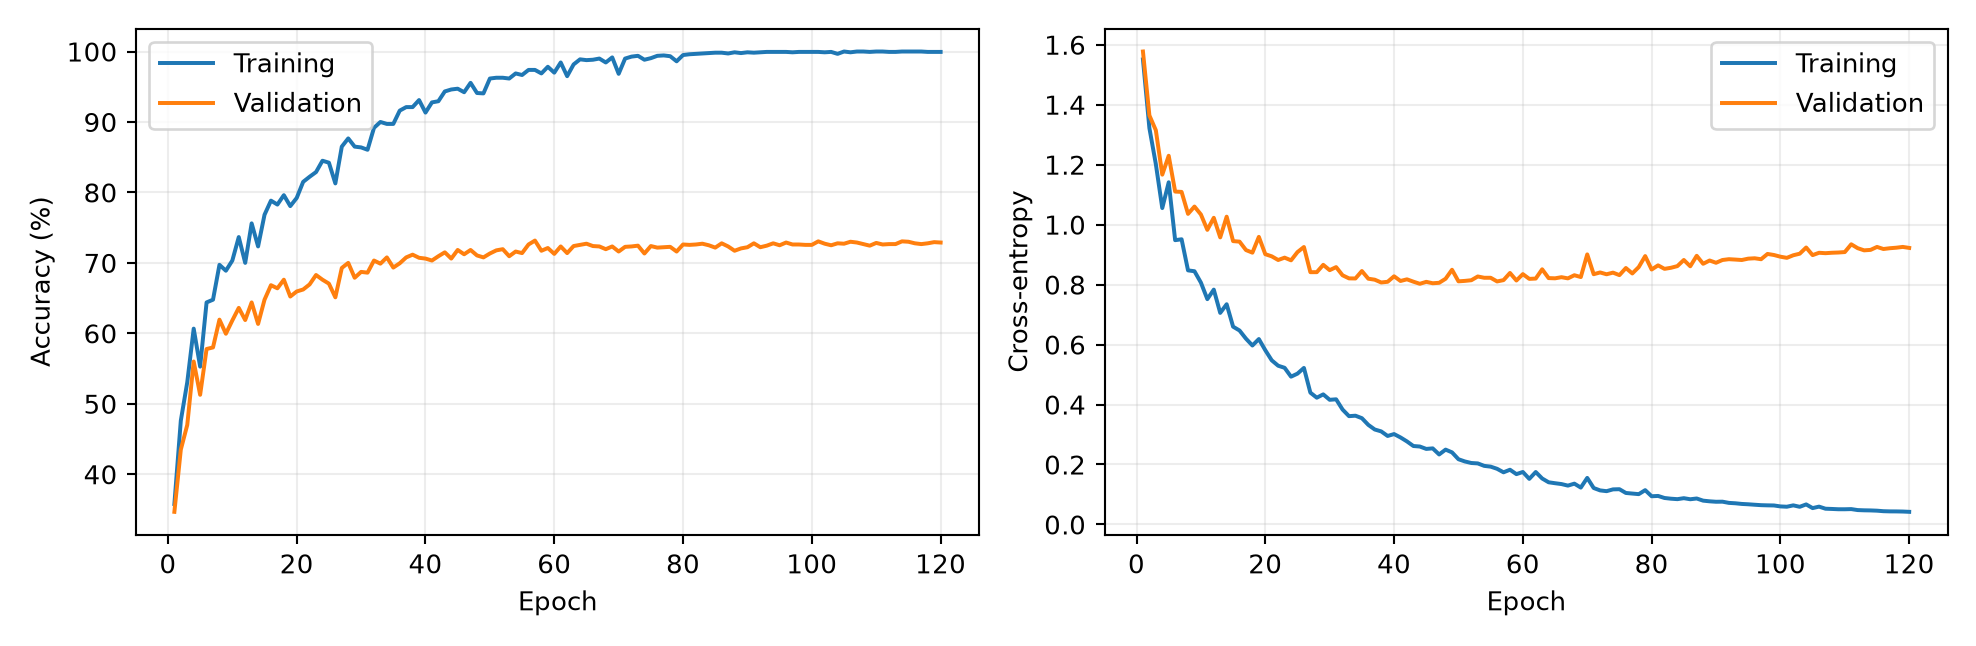
\includegraphics[width=1.0000\linewidth]{results/figures/D_large_curves.png}

\caption{Training and validation curves for the unregularized Large model.}
\end{figure}

Tiny has both low training accuracy and low validation accuracy, suggesting insufficient capacity within this budget. Small improves both. Medium and Large nearly fit the training set, yet finish with validation accuracy only slightly above Small and with worse validation cross-entropy. Large reaches 99.94\% training accuracy against 72.89\% validation accuracy. Its training CE continues down while validation CE turns upward: capacity alone is not enough. The growing loss gap also shows why accuracy by itself can conceal worsening confidence on errors.


\section{Part E - Effect of L2 Regularization}

The model is 24-128-128-6 with ReLU, cross-entropy, Kaiming normal initialization and learning rate 0.03. The SGD weight-decay value applies to \textbf{all trainable parameters, including biases}, as required. Every run uses the same initial parameters and batch sequence.


\begin{figure}[htbp]
\centering
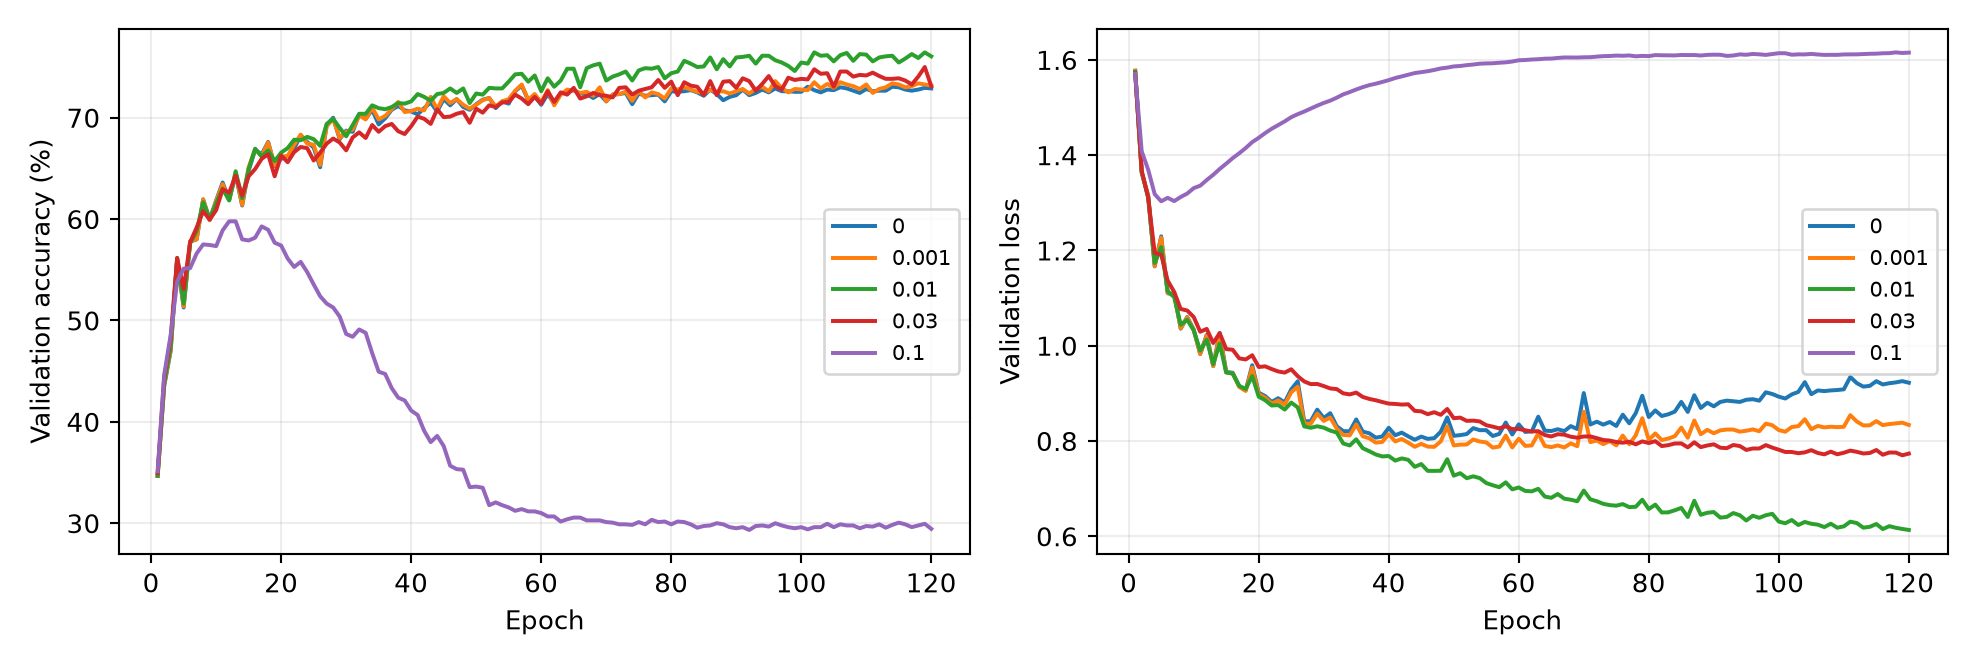
\includegraphics[width=1.0000\linewidth]{results/figures/E_decay.png}

\caption{Validation accuracy and cross-entropy for the five required weight-decay values.}
\end{figure}

\begin{table}[htbp]
\centering
\setlength{\tabcolsep}{4pt}
\renewcommand{\arraystretch}{1.12}
\small
\begin{tabular}{@{}>{\raggedright\arraybackslash}p{69.70pt} >{\raggedright\arraybackslash}p{98.41pt} >{\raggedright\arraybackslash}p{98.41pt} >{\raggedright\arraybackslash}p{73.81pt} >{\raggedright\arraybackslash}p{78.95pt}@{}}
\hline
Weight decay & Final train acc. (\%) & Final val. acc. (\%) & Final val. CE & Weight L2 norm \\
\hline
0 & 99.94 & 72.89 & 0.922 & 25.485 \\
0.001 & 99.94 & 73.17 & 0.834 & 23.367 \\
0.01 & 95.94 & 76.06 & 0.613 & 12.092 \\
0.03 & 81.94 & 73.11 & 0.773 & 6.336 \\
0.1 & 31.50 & 29.44 & 1.615 & 1.785 \\
\hline
\end{tabular}
\caption{Regularization results at epoch 120. The weight norm excludes biases.}
\end{table}

The reported weight norm is sqrt(sum over all weight-matrix entries of w\textsuperscript{2}), excluding biases. It is one norm of the concatenated weight matrices, rather than the sum of the individual layer norms. Biases are still regularized by the optimizer.


With no decay or 0.001, the model fits almost all training examples while validation CE rises late in training. Decay 0.01 reduces the final weight norm from 25.485 to 12.092, improves validation accuracy from 72.89\% to 76.06\%, and reduces validation CE from 0.922 to 0.613. This is the most useful balance among the five prescribed values.


Decay 0.03 reduces the gap further but also reduces training accuracy to 81.94\%; its final validation accuracy is 73.11\%. At 0.1 the weight norm falls to 1.785 and both datasets perform poorly. Its early validation peak does not persist: by epoch 120 it is clearly underfitting. The experiment supports moderate regularization for this model, rather than either no regularization or the strongest available value.


\section{Final Model Selection}

Parts A-E point to ReLU, cross-entropy, fan-in-scaled initialization and moderate weight decay. The extension first compared ReLU/Kaiming and tanh/Nielsen at hidden widths 32, 64-32, 128-128 and 128-64-32, with learning rate 0.03 and decay 0.001 or 0.01 (16 additional runs). Tanh did not match the leading ReLU models.


A focused follow-up used the two leading distinct architectures (128-128 and 64-32). It checked learning rates 0.01 and 0.05 with decay 0.01 or 0.03, plus rate 0.03 with decay 0.005 or 0.02. Six further checks used ReLU/Nielsen with widths 64, 128 or 128-128 and decay 0.01 or 0.03 at rate 0.03. These 18 follow-up runs used the same seed, batch size and 120-epoch budget; no prohibited optimizer or architecture was introduced.


\begin{table}[htbp]
\centering
\setlength{\tabcolsep}{4pt}
\renewcommand{\arraystretch}{1.12}
\small
\begin{tabular}{@{}>{\raggedright\arraybackslash}p{63.10pt} >{\raggedright\arraybackslash}p{59.16pt} >{\raggedright\arraybackslash}p{35.49pt} >{\raggedright\arraybackslash}p{39.44pt} >{\raggedright\arraybackslash}p{55.21pt} >{\raggedright\arraybackslash}p{78.88pt} >{\raggedright\arraybackslash}p{71.99pt}@{}}
\hline
Hidden layers & Init. & LR & Decay & Best epoch & Val. acc. (\%) & Val. CE \\
\hline
128-128 & Nielsen & 0.03 & 0.01 & 106 & 77.39 & 0.596 \\
128-128 & Kaiming & 0.03 & 0.02 & 106 & 77.39 & 0.669 \\
128-128 & Kaiming & 0.05 & 0.01 & 116 & 77.33 & 0.587 \\
64-32 & Kaiming & 0.05 & 0.01 & 107 & 77.00 & 0.599 \\
128-128 & Kaiming & 0.03 & 0.01 & 119 & 76.44 & 0.615 \\
64-32 & Kaiming & 0.03 & 0.02 & 106 & 76.44 & 0.689 \\
64-32 & Kaiming & 0.03 & 0.01 & 119 & 75.83 & 0.632 \\
\hline
\end{tabular}
\caption{Leading distinct configurations, ranked by validation accuracy and then cross-entropy.}
\end{table}

\begin{figure}[htbp]
\centering
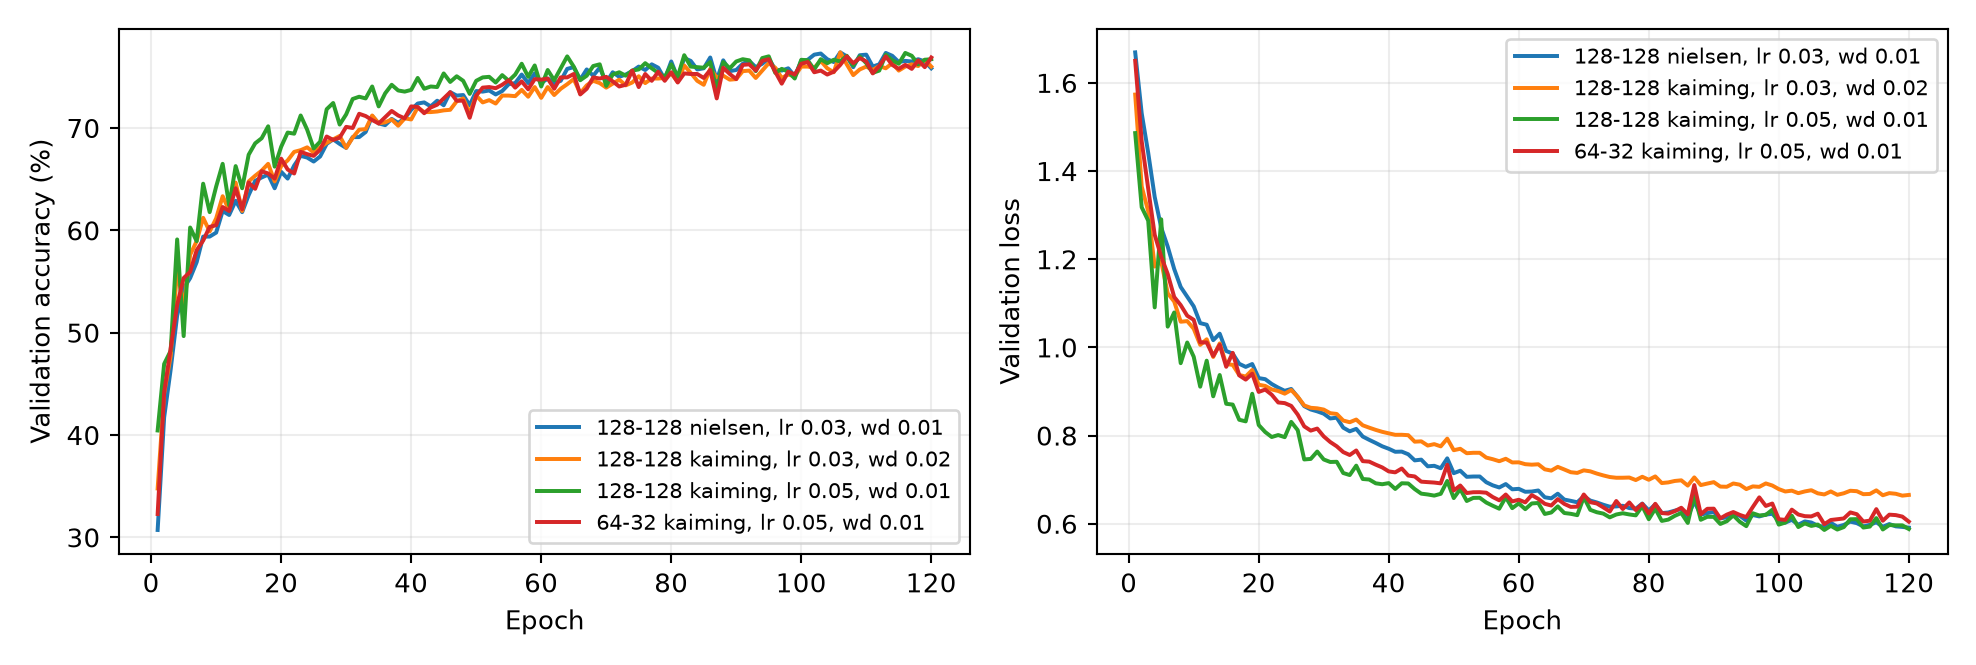
\includegraphics[width=1.0000\linewidth]{results/figures/search_leaders.png}

\caption{Full validation curves for the leading configurations; isolated accuracy peaks are small relative to the overall trends.}
\end{figure}

The two leading configurations tie at 77.39\% accuracy. The Nielsen model has lower cross-entropy (0.596 versus 0.669), so the selected architecture is \textbf{24-128-128-6} with \textbf{ReLU, Nielsen initialization, learning rate 0.03 and weight decay 0.01}. A smaller 64-32 model reaches 77.00\%, so the advantage of the larger model is modest. The six-digit seed remains fixed; no seed search, ensemble, parameter averaging or learning-rate schedule was used. Validation has been used repeatedly for selection, so these scores should not be treated as unbiased estimates of hidden-test performance.


\section{Training Duration at a Larger Dataset Size}

After fixing the architecture and all other hyperparameters, training duration was checked using four larger-data folds. The 1,800 original training examples remain in every fold. The validation rows are shuffled with seed 831031 into four groups of 450. Each fold trains on the original training rows plus 1,350 validation rows and holds out the remaining 450 rows: 3,150 training examples per fold. No held-out labels are used in its gradient updates.


All four models start from scratch and train for 120 epochs. Input scaling stays fixed to the original training.csv statistics, because the original training rows are present in every fold. The mean held-out accuracy across folds selects the duration; ties use mean held-out cross-entropy, then the earlier epoch. No setting other than duration is adjusted here.


\begin{figure}[htbp]
\centering
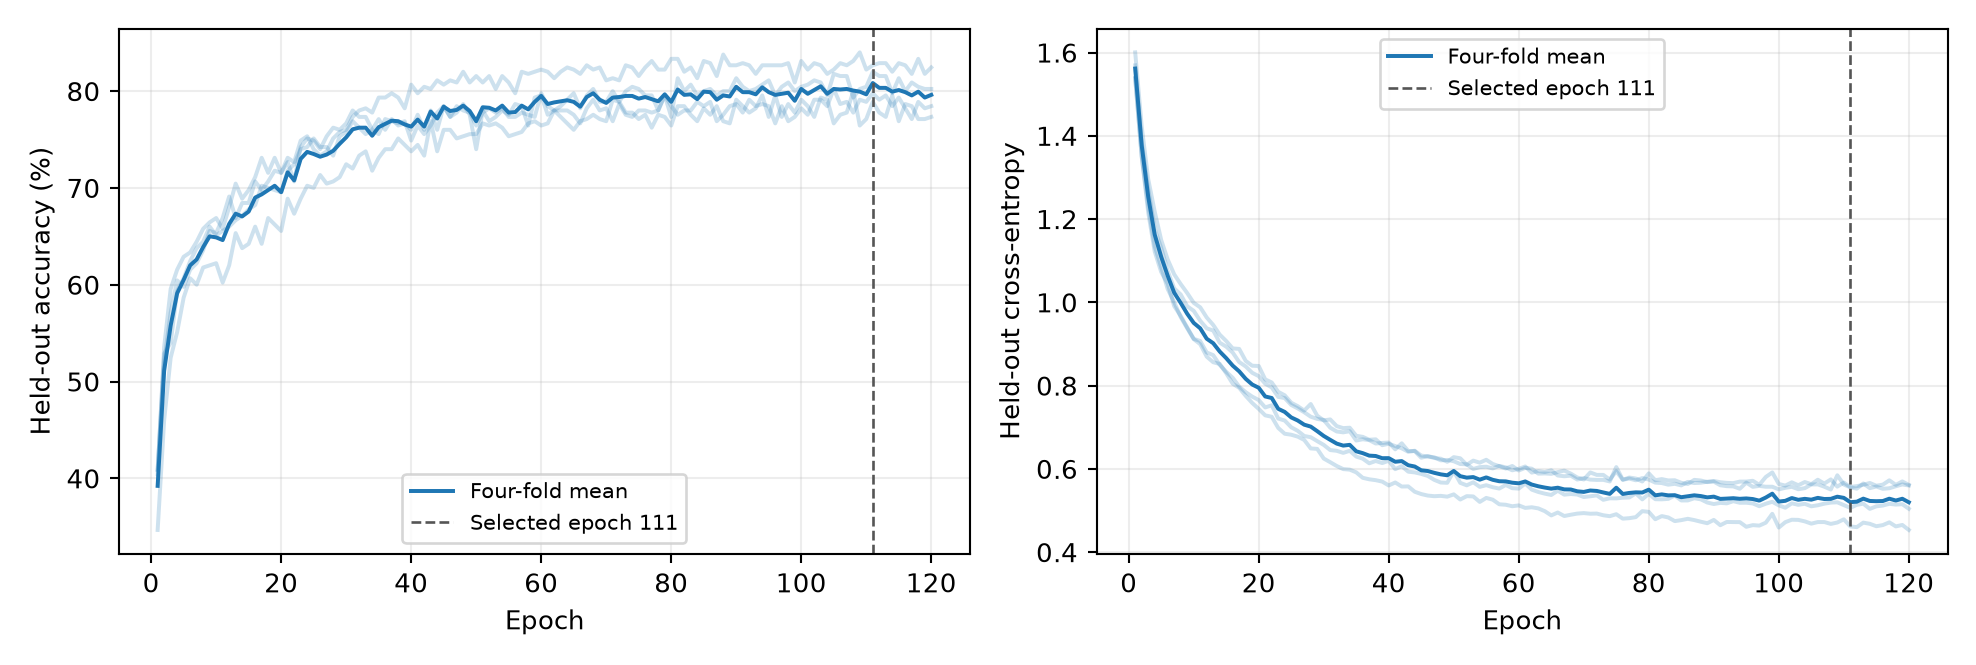
\includegraphics[width=1.0000\linewidth]{results/figures/larger_data_diagnostic.png}

\caption{Faint lines show individual folds; solid lines show the four-fold mean. The dashed line marks the selected epoch.}
\end{figure}

\begin{table}[htbp]
\centering
\setlength{\tabcolsep}{4pt}
\renewcommand{\arraystretch}{1.12}
\normalsize
\begin{tabular}{@{}>{\raggedright\arraybackslash}p{63.85pt} >{\raggedright\arraybackslash}p{208.58pt} >{\raggedright\arraybackslash}p{162.84pt}@{}}
\hline
Epoch & Mean held-out accuracy (\%) & Mean held-out CE \\
\hline
30 & 75.22 & 0.679 \\
60 & 79.50 & 0.565 \\
90 & 80.44 & 0.533 \\
106 & 80.17 & 0.530 \\
111 & 80.83 & 0.520 \\
120 & 79.61 & 0.520 \\
\hline
\end{tabular}
\caption{Mean held-out performance in the four-fold duration diagnostic.}
\end{table}

The selected duration is \textbf{111 epochs}, at mean held-out accuracy \textbf{80.83\%} and CE 0.520. The sample standard deviation of accuracy across the four folds is 1.79 percentage points. The original 1,800-row search had its best checkpoint at epoch 106; the larger-data diagnostic supports a nearby duration rather than an unrestricted extension beyond the assignment budget.


This is a model-selection diagnostic, not a new independent test. Architecture and hyperparameters were already chosen using the supplied validation set. The folds also share many training rows. Their mean is useful for choosing a duration at a training size closer to 3,600, but it does not remove the optimism caused by earlier validation-based selection.


\section{Validation Confusion Matrix}

To evaluate the fully selected configuration, a fresh model was trained on the original 1,800 training rows for exactly 111 epochs. This duration was fixed by the larger-data diagnostic; no new checkpoint selection was made from this run. Its training accuracy is 94.67\% and validation accuracy is \textbf{76.00\%} (1368 of 1800 examples). Training and validation CE are 0.298 and 0.605.


\begin{figure}[htbp]
\centering
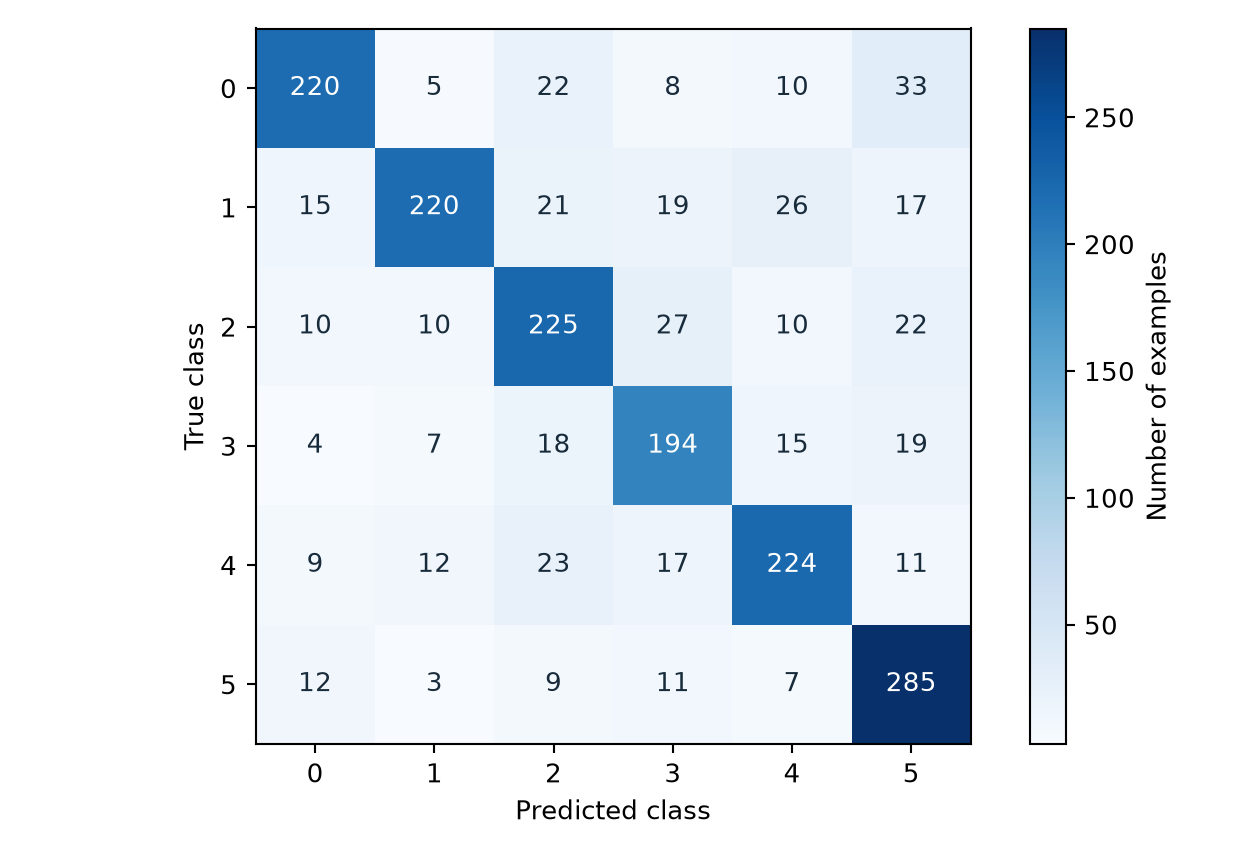
\includegraphics[width=0.7139\linewidth]{results/figures/validation_confusion.png}

\caption{Confusion matrix on the original validation.csv. Rows are true labels and columns are predictions.}
\end{figure}

\begin{table}[htbp]
\centering
\setlength{\tabcolsep}{4pt}
\renewcommand{\arraystretch}{1.12}
\small
\begin{tabular}{@{}>{\raggedright\arraybackslash}p{36.20pt} >{\raggedright\arraybackslash}p{128.71pt} >{\raggedright\arraybackslash}p{52.29pt} >{\raggedright\arraybackslash}p{52.29pt} >{\raggedright\arraybackslash}p{68.37pt} >{\raggedright\arraybackslash}p{73.42pt}@{}}
\hline
Class & Operating condition & Support & Correct & Recall (\%) & Precision (\%) \\
\hline
0 & Normal & 298 & 220 & 73.83 & 81.48 \\
1 & Condition A & 318 & 220 & 69.18 & 85.60 \\
2 & Condition B & 304 & 225 & 74.01 & 70.75 \\
3 & Condition C & 257 & 194 & 75.49 & 70.29 \\
4 & Condition D & 296 & 224 & 75.68 & 76.71 \\
5 & Condition E & 327 & 285 & 87.16 & 73.64 \\
\hline
\end{tabular}
\caption{Per-class results for the selected original-split validation model.}
\end{table}

Class 5 is the most reliably recovered by recall (87.16\%). Class 1 has the lowest recall (69.18\%). The largest directional confusion is true class 0 predicted as 5: 33 examples (11.07\% of class 0). These counts show where the remaining errors concentrate; they do not establish a physical explanation because the sensor features and operating conditions are anonymized.


This 111-epoch original-split score differs from the 77.39\% search peak at epoch 106. Both are reported explicitly: the architecture comes from the search, while the final duration comes from the larger-data diagnostic. The confusion matrix is from the original split before merging, not from a model that has already trained on validation.csv.


\section{Final Model Training and Export}

\begin{table}[htbp]
\centering
\setlength{\tabcolsep}{4pt}
\renewcommand{\arraystretch}{1.12}
\normalsize
\begin{tabular}{@{}>{\raggedright\arraybackslash}p{125.71pt} >{\raggedright\arraybackslash}p{317.56pt}@{}}
\hline
Final setting & Selected value \\
\hline
Architecture & 24-128-128-6 (20,486 trainable parameters) \\
Hidden activation / output & ReLU in both hidden layers / six logits \\
Initialization / biases & Nielsen normal, standard deviation 1/sqrt(fan-in) / zero biases \\
Loss / optimizer & Cross-entropy / SGD without momentum \\
Learning rate / mini-batch & 0.03 / 64 \\
Weight decay & 0.01 on all weights and biases \\
Epochs / seed & 111 / 831031 \\
Training data & All 3,600 supplied examples \\
Normalization & Original training.csv statistics only; no recomputation after merging \\
\hline
\end{tabular}
\caption{Final model configuration.}
\end{table}

All model choices were fixed before final retraining. A new model was initialized from scratch and trained on the combined, already-standardized rows for the selected number of epochs. The final weights are from the last epoch of that run. No combined-data metric was used for another round of model or epoch selection.


At the final epoch, combined-data training accuracy is \textbf{91.86\%} and cross-entropy is \textbf{0.341}. These are training diagnostics. A checker score on the original validation rows is also an in-sample sanity check now that those rows were included in final training; it is not a new generalization estimate.


\subsection*{Export checks}

The provided save\_model\_json.py helper writes the architecture, activation, weight matrices and biases in x1 through x24 feature order. Reloading the JSON gives bitwise identical PyTorch logits on all 3,600 standardized examples. The supplied check\_model\_json.py accepts the exported file. Additional checks confirm zero initial biases, identical starting parameters for Parts A and B, identical histories for repeated controlled configurations, and unchanged training-only preprocessing. All losses and parameters are finite. No PA1 test data were used in any PA2 experiment.


\section{Conclusion}

Nonlinearity is useful on this task, but the activation and initialization affect how quickly the model learns within a fixed budget. Cross-entropy gives better accuracy than quadratic cost under the prescribed comparison. Larger models fit the training data much more closely, so their additional capacity needs regularization. Moderate decay improves the validation result; excessive decay removes useful capacity. The final choice combines this evidence with a held-out duration check at a larger training-set size. The hidden 50,000-example test set was unavailable, so no hidden-test accuracy or mark is claimed.


\section{Generative-AI Assistance Acknowledgement}

OpenAI Codex assisted with implementation, experiment execution, analysis, figures and report drafting. The numerical results and plots were produced by running the program on the supplied CSV files; the export was verified with the supplied checker.


\section{References}

1. BITS F445, Programming Assignment 2 question paper and supporting scripts.\newline 2. PyTorch 2.14 documentation: \href{https://docs.pytorch.org/docs/2.14/generated/torch.nn.CrossEntropyLoss.html}{CrossEntropyLoss}, \href{https://docs.pytorch.org/docs/2.14/generated/torch.optim.SGD.html}{SGD}, and \href{https://docs.pytorch.org/docs/2.14/nn.init.html}{weight initialization}.\newline 3. Michael Nielsen, Neural Networks and Deep Learning, Chapter 3 (quadratic cost convention).

\end{document}
